\documentclass[../Bachelorarbeit.tex]{subfiles}
\begin{document}

\subsection{Anwendungsfallspezifikation}
Nach dem Abschließen der Festlegung des Kontextes des mehrachsigen Positioniersystems folgt nun die Identifizierung von Systemprozessen. Der Findungsprozess erfolgt über die Anwendungsfallanalyse. Dabei wird ein System als Black-Box betrachtet, um möglichst gute Systemprozesse zu finden, ohne sich von internen Gegebenheiten des Systems beeinflussen zu lassen.\\ % Quelle
Die Anwendungsfallspezifikation wird in dieser Arbeit in zwei Unterkapitel eingeteilt. Ersteres beschäftigt sich mit dem Finden und Entwickeln von Systemprozesses. Das zweite Unterkapitel hat zum Ziel die Systemprozesse zu präzisieren und diese dann übersichtlich darzustellen.\\

\subsubsection{Entwicklung der Systemprozesse}
Die Anwendungsfallanalyse baut auf dem Anwendungsfalldiagramm aus \autoref{fig:my-img1} auf. Dabei findet auch an dieser Stelle eine Unterteilung in zwei Abschnitte statt. Im ersten Schritt werden die Akteure aus den Diagrammen des \autoref{kontextana} geprüft und um eventuelle Akteure ergänzt, die bis zu diesem Zeitpunkt nicht erkannt wurden. Diese werden zunächst in die Kontextabgrenzung mit aufgenommen, bevor im folgenden Abschnitt die Anwendungsfallanalyse beginnt.\\
Im zweiten Schritt werden die Erwartungen der Akteue an das System untersucht. Aus dieser Analyse erfolgt die Ableitunge von möglichen Systemprozessen. Dieser Abschnitt hat es folglich als Ziel, die Frage nach den durch die Akteure geforderten Voraussetzungen zu beantworten.\\
Für die Entwicklung der Systemprozzesse wird folglich auf den logischen Kontext zurückgegriffen, da dieser dieser die Akteure des Systems bereits im Anwendungsfalldiagramm (siehe \autoref{fig:my-img1}) zeigt. Da es an dieser Stelle nur um die Frage nach den Akteuren und ihren Erwartungen geht und dabei die Hardware und die Ausprägung der Kommunikation des Positioniersystems nicht relevant ist, spielen der physikalische Kontext und dessen Ergebnisse keine Rolle.\\
Die \autoref{fig:my-img3} zeigt die Systemprozesse, die aus der Anlagenbeschreibung modelliert werden. Es ist ersichtlich, dass gezeigtes Anwendungsfalldiagramm eine Erweiterung der \autoref{fig:my-img1} aus dem vorhergegangenen Unterabschnitt ist.\\
Neu daszugekommen sind die Anwendungsfälle, die durch den Anlagennutzer ausgelöst werden können. Konkret handelt es sich also um die zwei auswählbaren Betriebsmodi und den Not-Halt. Weiterhin ist der Transport von Gegenständen im Anwendungsfalldiagramm aufgeführt. Es handelt sich dabei um den grundsätzlichen Nutzen des Positioniersystems. Es ist wichtig zu berücksichtigen, dass dieser Anwendungsfall von den vorher genannten drei Anwendungsfällen/Betriebszuständen abhängig ist. Zuletzt findet sich noch die Bereitstellung von Prozessdaten im Diagramm wieder.

\begin{figure}[h]
    \centering
    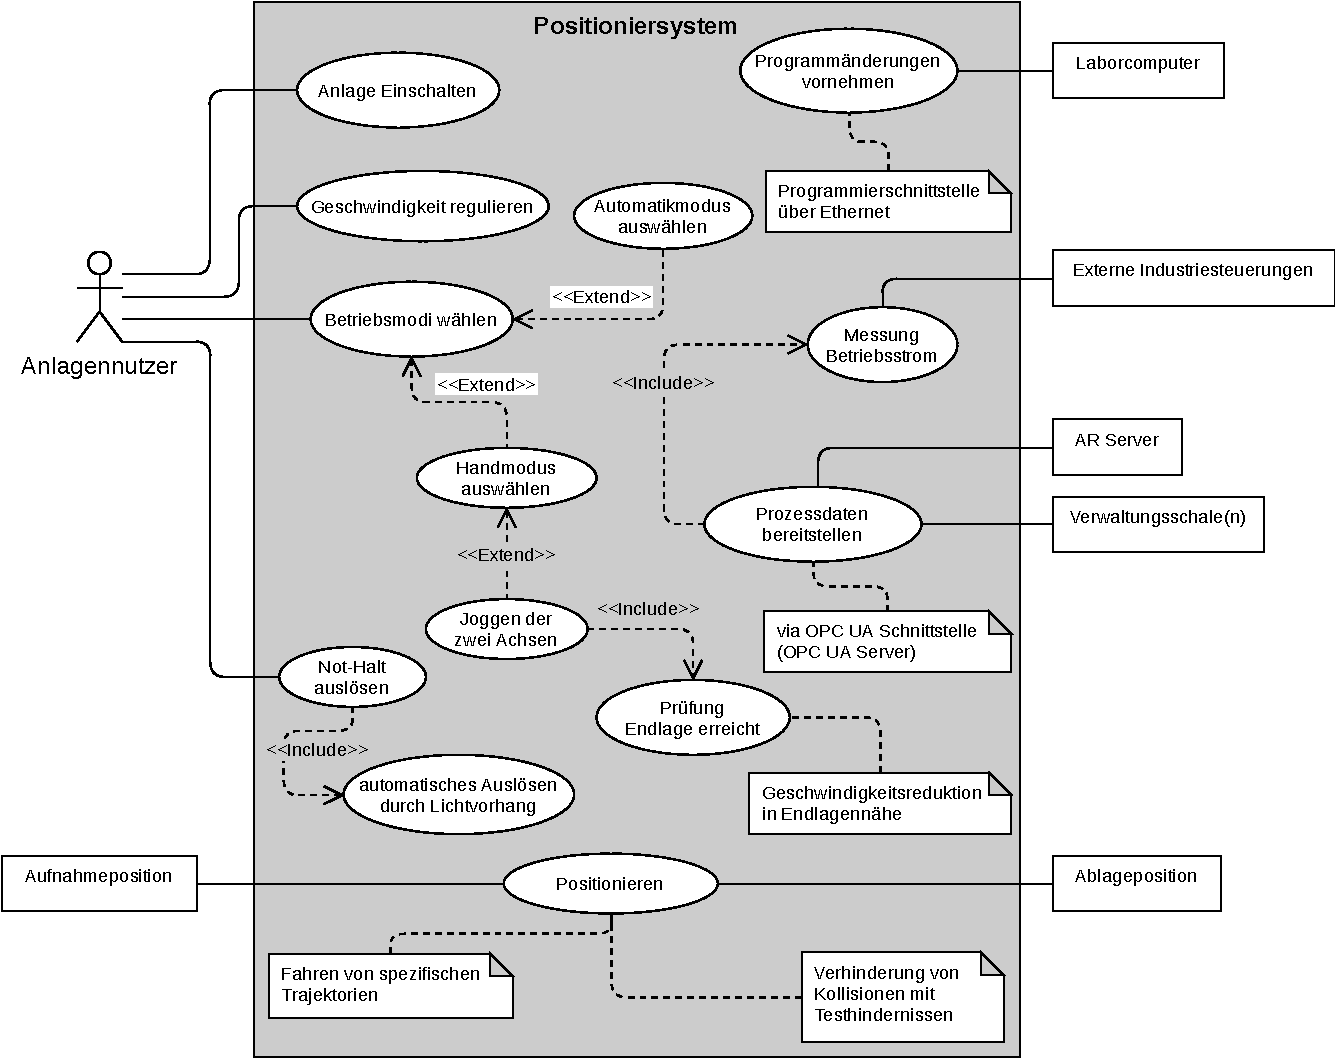
\includegraphics[width=\textwidth]{Images/use_case_dia.pdf}
    \caption[Anwendungsfalldiagramm]{Anwendungsfalldiagramm des Positioniersystems}
    \label{fig:my-img3}
\end{figure}



\subsubsection{Präzisierung der Systemprozesse}

\end{document}